\section{Simulation und Ergebnisse} % (fold)
\label{sec:simulation_und_ergebnisse}

	
	\subsection{Ausgabe und Visualisierung} % (fold)
	\label{sub:ausgabe_und_visualisierung}
	
		Für die Visualisierung wurde mithilfe der Bibliothek \textit{Qt v5.1.1} eine Klasse erstellt, welche durch die Übergabe eines diskretisierten Vektorfeldes, dieses automatisch darstellt.
		Dabei wird eine bestimmte Anzahl an Position zufällig gewählt.
		An diesen Position werden dann Teilausschnitte der Strömungslinien des Vektorfeldes angezeigt.
		Die Länge stellt ein natürliches Maß für die Stärke des Vektorfeldes an den jeweiligen Punkten dar.
		In Abbildung \ref{fig:example view} ist als Beispiel das folgende Vektorfeld $\vec{v}$ auf dem Bereich $[0,1]^2$ dargestellt worden.
		\[ \vec{v}(x,y) := x\vec{e_x} + \sqrt{x}\sin(3\pi x)\sin(\pi y)\vec{e_y} \]

		\begin{figure}[!htb]
			\center
			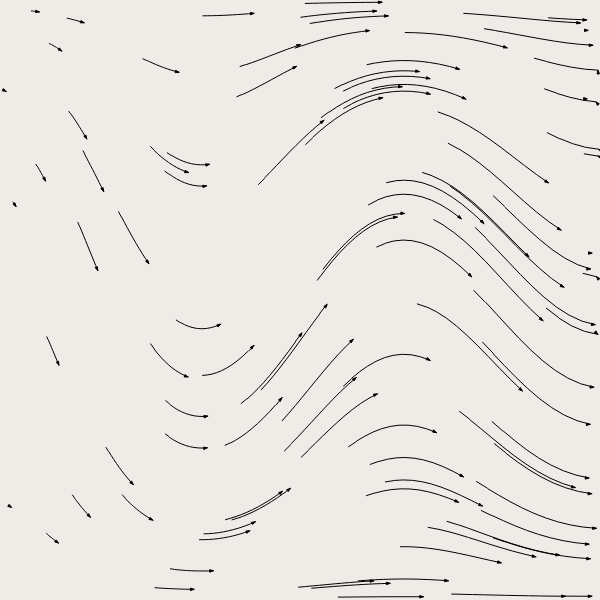
\includegraphics[scale = 0.35]{screenshots/example-01.png}
			\caption{Visualisierung des Beispielvektorfeldes $\vec{v}$ durch das erstellte Programm. \\ Vergleiche mit \cite{nsfd}.}
			\label{fig:example view}
		\end{figure}

		Für diskretisierte skalare Felder, wie den Druck, ist die selbe Klasse zuständig.
		Dabei werden verschiedene Farbwerte verwendet um die Stärke des Feldes zu verdeutlichen.
		Im Programm selbst wurden stärkere Werte durch rötlichere Farben und schwächere durch bläuliche Farben dargestellt.
		Als Beispiel sei die Visualisierung des skalaren Feldes $v_y$ durch das Programm in Abbildung \ref{fig:example view scalar} gegeben.

		\begin{figure}[!htb]
			\center
			
\includegraphics[scale = 0.35]{screenshots/example-02.png}
			\caption{Visualisierung des skalaren Feldes $v_y$ durch das Programm. \\ Vergleiche mit \cite{nsfd}.}
			\label{fig:example view scalar}
		\end{figure}

	% subsection ausgabe_und_visualisierung (end)

	\subsection{Zeitevoluion einer Flüssigkeit} % (fold)
	\label{sub:zeitevoluion_einer_fl_ssigkeit}
	
		Im Folgenden wurden für das Programm die unten stehenden Parameter verwendet.
		\[ Re = 100 \quad u = 1.28 \quad i_{max} = 64 \quad j_{max} = 64 \]
		\[ a=b=1.0 \quad \tau = 0.5 \quad \gamma = 0.5 \quad \epsilon = 0.001 \quad \omega = 0.5 \]
		Diese Parameter werden beibehalten, sollte keine weitere Angabe zu Ihnen erfolgen.

		Die Nischenströmung konnte mithilfe des Programmes erfolgreich simuliert werden.
		Es wurden für vier verschiedene Zeiten die Evolution der Flüssigkeit in der Zelle aufgenommen.
		Diese sind in Abbildung zu sehen.

		\begin{figure}[!htb]
			\begin{subfigure}[b]{.5\textwidth}
				\center
				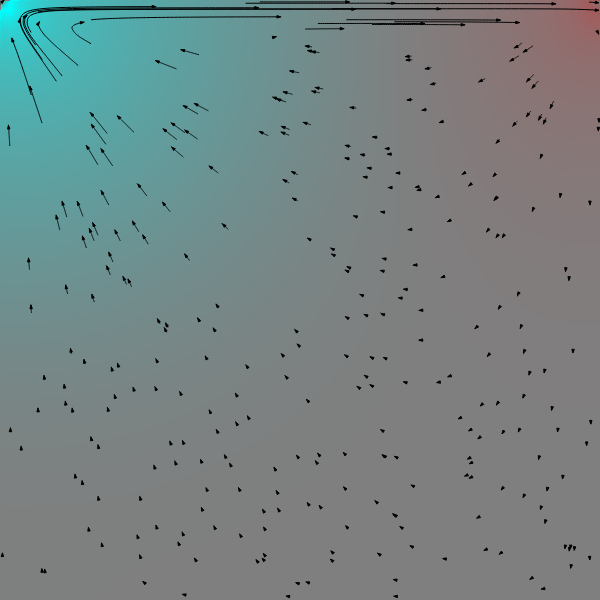
\includegraphics[scale=0.28]{screenshots/time-0030.png}
				\caption{$t=0.03$}
				\label{fig:time 01}
			\end{subfigure}
			\begin{subfigure}[b]{.5\textwidth}
				\center
				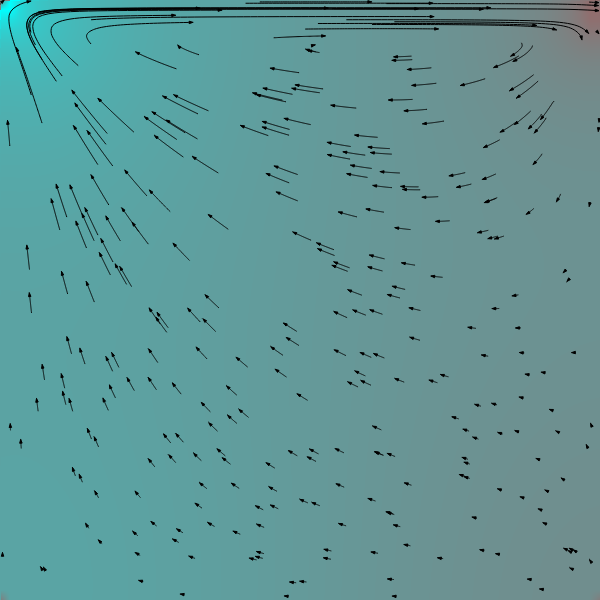
\includegraphics[scale = 0.28]{screenshots/time-0060.png}
				\caption{$t=0.06$}
				\label{fig:time 02}
			\end{subfigure}
			\begin{subfigure}[b]{.5\textwidth}
				\center
				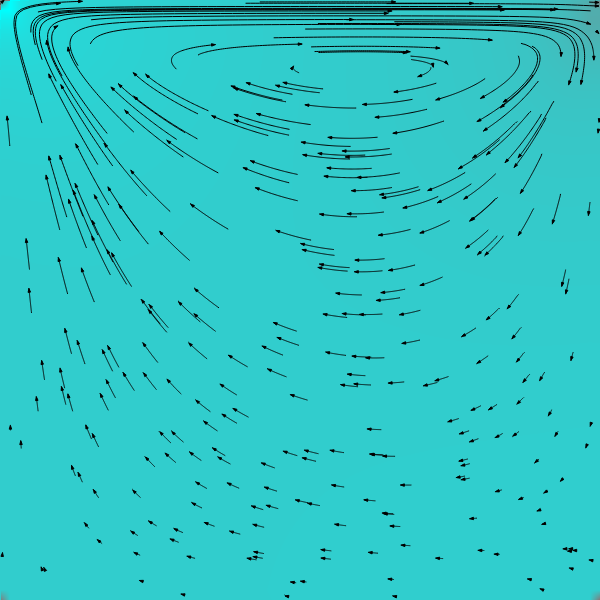
\includegraphics[scale = 0.28]{screenshots/time-0200.png}
				\caption{$t=0.2$}
				\label{fig:time 03}
			\end{subfigure}
			\begin{subfigure}[b]{.5\textwidth}
				\center
				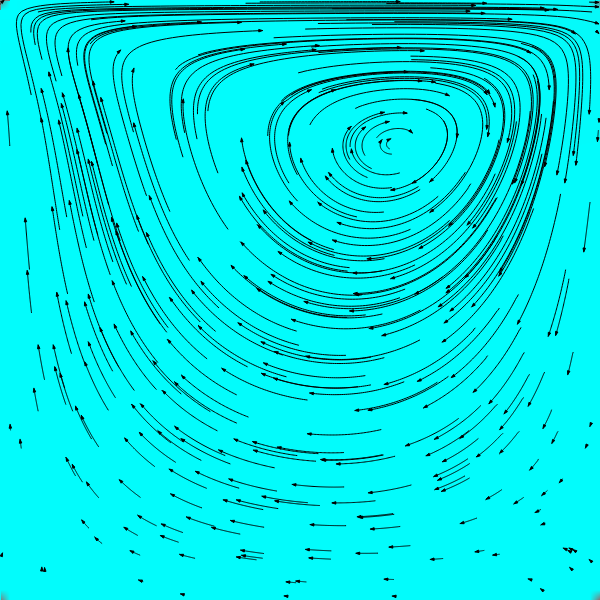
\includegraphics[scale = 0.28]{screenshots/time-3800.png}
				\caption{$t=3.8$ (stationärer Endzustand)}
				\label{fig:time 04}
			\end{subfigure}
			\caption{simulierte Zeitevolution des Geschwindigkeits- und Druckfeldes für $Re = 100$}
			\label{fig:time evolution}
		\end{figure}

		Diese Ergebnisse entsprechen den Ergebnissen aus \cite{nsfd} und decken sich mit der Erfahrung.
		Zu Beginn sind deutliche Druckunterschiede zu beobachten.
		Im oberen rechten Bereich entsteht durch die Aufstauung der Flüssigkeit an der rechten Wand eine Druckerhöhung.
		Analog dazu lässt sich der Druck im linken Bereich durch einen Sog erklären.
		Im Laufe der Zeit gleichen sich die Druckunterschiede aus, da die Flüssigkeit inkompressibel ist.
		Im stationären Endzustand, der nach circa $3.5\unit{s}$ erreicht war, ist der Druck im gesamten Bereich minimal (hellblaue Farbe).

		Das Geschwindigkeitsfeld bildet bereits kurz nach dem Start der Simulation einen Wirbel aus.
		Dieser ist zuerst, wie in Abbidung zu erkennen, sehr flach im oberen Bereich zu sehen.
		Mit der Zeit wird die gesamte träge Flüssigkeit aufgrund innerer Reibung beschleunigt.
		Der Wirbel wird größer bis er im Endzustand fast die gesamte Zelle einnimmt.
		Dabei verschiebt sich das Zentrum des Wirbels leicht nach rechts.
		Aufgrund der nicht rotationssymmetrischen Boxgeometrie kommt es zu Deformierungen des Wirbels an den Ecken der Zelle.
		In den unteren beiden Ecken der Zellen sind die Beträge des Geschwindigkeitsfeldes zu gering, um eine nähere Untersuchung zuzulassen.
		Es lässt sich jedoch erkennen, dass der Wirbel dort abbricht.

		In der rechten oberen Ecke verlassen einige Pfeile die Box.
		Dies würde den Haftbedingungen widersprechen.
		Jedoch sind diese Fehler auf numerische Rundungsfehler bei der Darstellung und endliche Ortsauflösung zurückzuführen, da die Gesamtlösung dadurch nicht verändert wird.

	% subsection zeitevoluion_einer_fl_ssigkeit (end)


	\subsection{Einfluss der Reynoldszahl} % (fold)
	\label{sub:einfluss_der_reynoldszahl}

		Die Simulationen wurden nun mit steigender Reynoldszahl durchgeführt.
		Alle weiteren Parameter wurden konstant gelassen.
		Im Folgenden sollen nur noch die stationären Endzustände der Geschwindigkeitsfelder betrachtet werden.

		Während für Reynoldszahlen von $1$ bis $10$ die Ergebnisse qualitativ gleich sind, erkennt eine deutliche Verschiebung und Deformierung des Wirbels ab $Re = 100$.
		Kleinere Reynoldszahlen bedeuten eine höhere Viskosität.
		In den ersten beiden Fällen ist also die innere Reibung der Flüssigkeiten so groß, dass asymmetrische Turbulenzen verhindert werden.

		\begin{figure}[!htb]
			\begin{subfigure}[b]{.5\textwidth}
				\center
				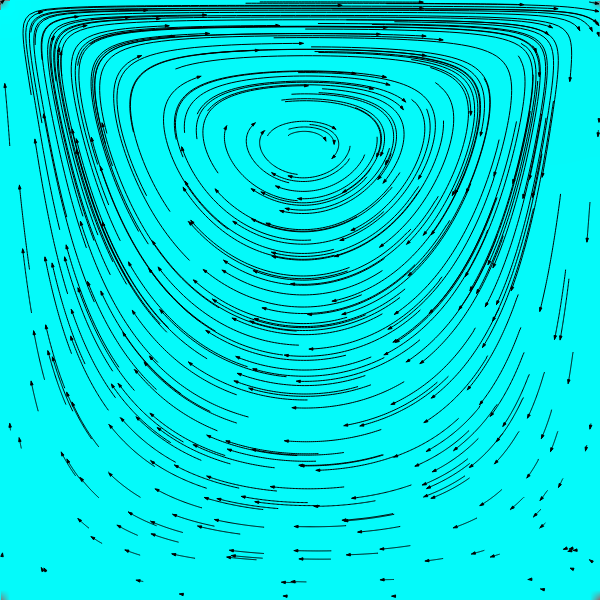
\includegraphics[scale = 0.28]{screenshots/re-1.png}
				\caption{$Re=1$}
				\label{fig:re 1}
			\end{subfigure}
			\begin{subfigure}[b]{.5\textwidth}
				\center
				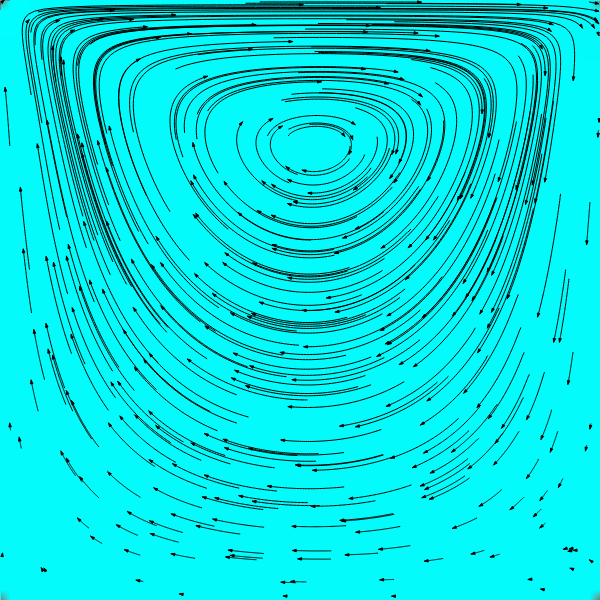
\includegraphics[scale = 0.28]{screenshots/re-10.png}
				\caption{$Re=10$}
				\label{fig:re 10}
			\end{subfigure}
			
			\begin{subfigure}[b]{.5\textwidth}
				\center
				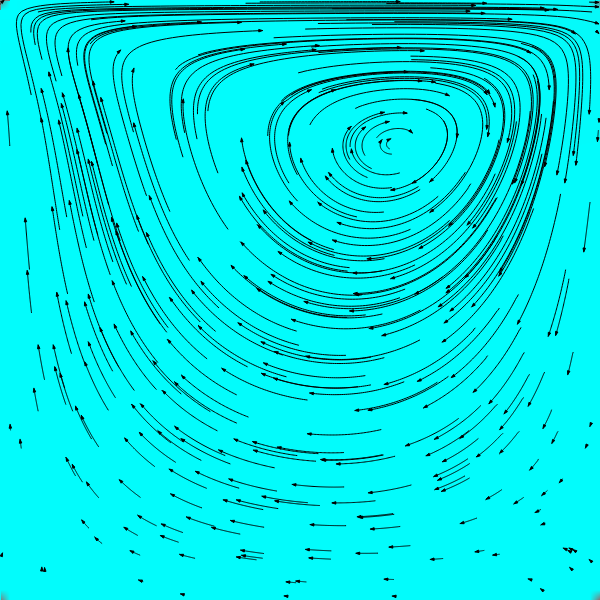
\includegraphics[scale = 0.28]{screenshots/time-3800.png}
				\caption{$Re=100$}
				\label{fig:re 100}
			\end{subfigure}
			\begin{subfigure}[b]{.5\textwidth}
				\center
				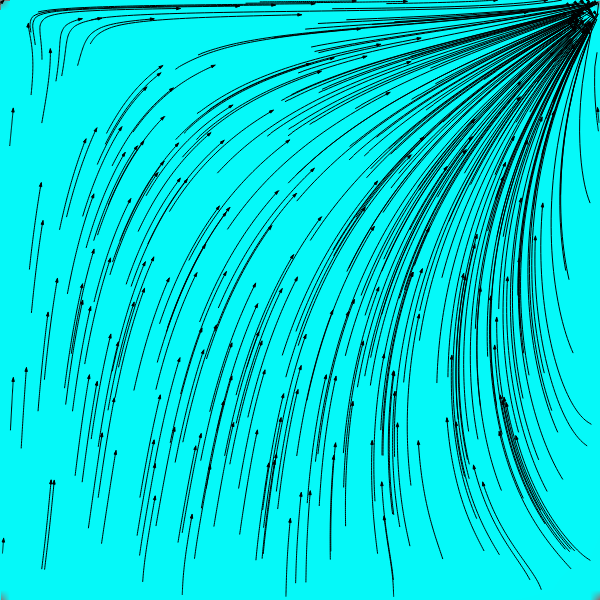
\includegraphics[scale = 0.28]{screenshots/re-1000-64.png}
				\caption{$Re=1000$}
				\label{fig:re 1000 64}
			\end{subfigure}
			\caption{simulierte Strömungslinien im stationären Endzustand für verschiedene Reynoldszahlen}
			\label{fig:steady state re}
		\end{figure}

		Im Falle von $Re = 1000$ ist deutlich erkennbar, dass ein Fehler in der Berechnung aufgetreten ist.
		Hier stößt man mit der Ortsauflösung von $64\times64$ Gitterpunkten und der daraus folgenden Zeitauflösung an die Grenzen der Simulation.
		In dem Programm wird eine $32$-bit Auflösung der reellen Zahlen verwendet.
		Diese besitzt eine relative Genauigkeit von rund $10^{-6}$.
		Mit einer $64$-bit Auflösung könnte in diesem Falle nun ein besseres Ergebnis erzielt werden.
		Auch eine zu groß gewählte Randgeschwindigkeit kann zu einer numerischen Instabilität führen.
		Für $Re=1000$ haben wir nun die Anzahl der Gitterpunkte auf $512\times 512$ erhöht und die Geschwindigkeit auf $1.0$ gesetzt.
		Es war somit möglich eine stabile numerische Berechnung zu realisieren.
		Dies ist jedoch mit einem erheblich größeren Rechen- und Zeitaufwand verbunden.
		Die genauen Ergebnisse der Simulation sind in den Abbildungen \ref{fig:time re 1000 1} und \ref{fig:time re 1000 2} zu sehen.
		Diese Zeitevolution stimmt mit den Ergebnissen aus \cite{nsfd} ohne Einschränkungen überein (siehe Anhang).

		\begin{figure}[!htb]
			\centering
			\begin{subfigure}[b]{.5\textwidth}
				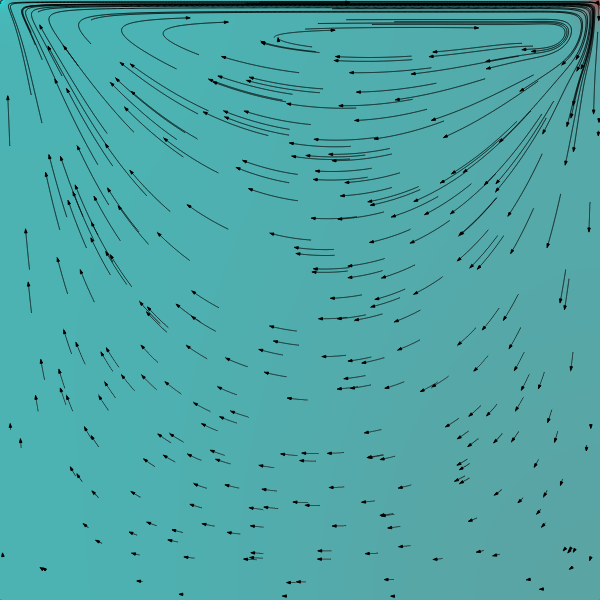
\includegraphics[scale = 0.28]{screenshots/re-1000-512-00520.png}
				\caption{$t=0.520$}
			\end{subfigure}%
			\begin{subfigure}[b]{.5\textwidth}
				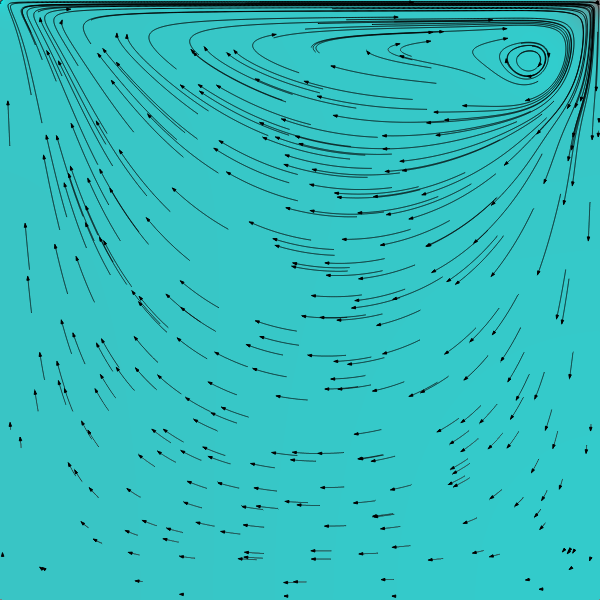
\includegraphics[scale = 0.28]{screenshots/re-1000-512-01069.png}
				\caption{$t=1.069$}
			\end{subfigure}

			\begin{subfigure}[b]{.5\textwidth}
				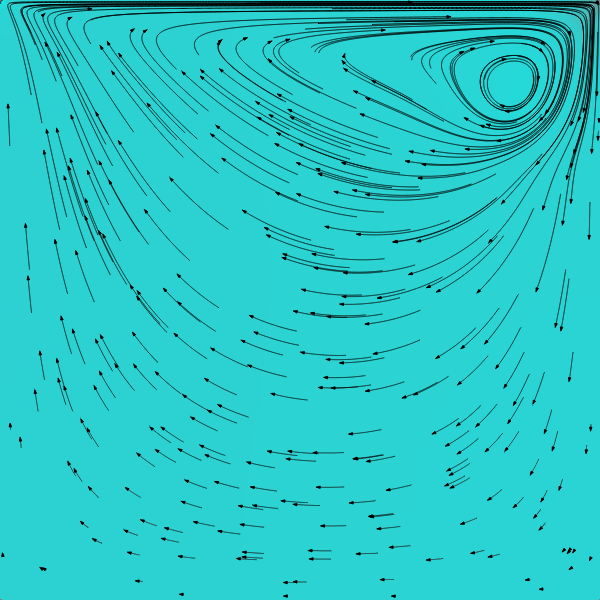
\includegraphics[scale = 0.28]{screenshots/re-1000-512-01555.png}
				\caption{$t=1.555$}
			\end{subfigure}%
			\begin{subfigure}[b]{.5\textwidth}
				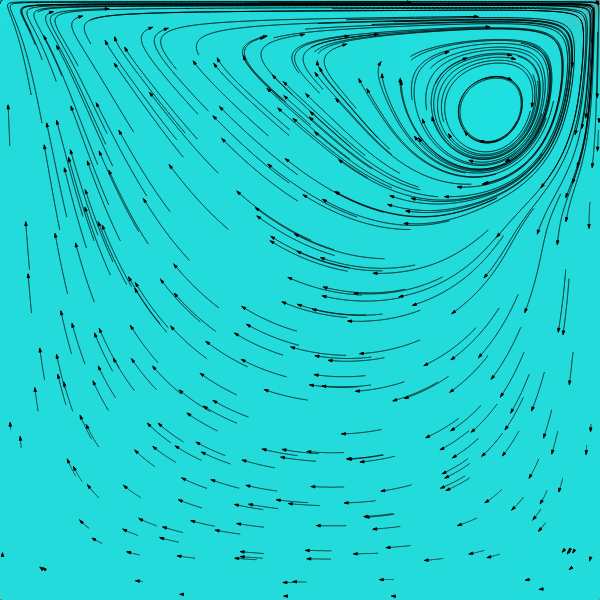
\includegraphics[scale = 0.28]{screenshots/re-1000-512-02170.png}
				\caption{$t=2.170$}
			\end{subfigure}

			\begin{subfigure}[b]{.5\textwidth}
				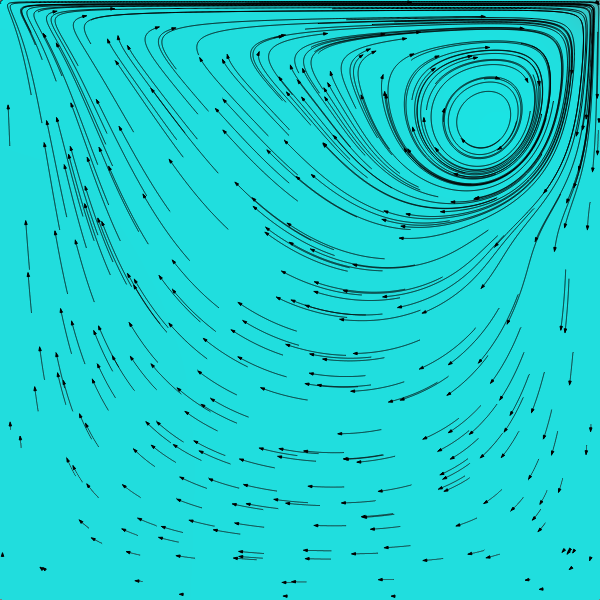
\includegraphics[scale = 0.28]{screenshots/re-1000-512-02405.png}
				\caption{$t=2.405$}
			\end{subfigure}%
			\begin{subfigure}[b]{.5\textwidth}
				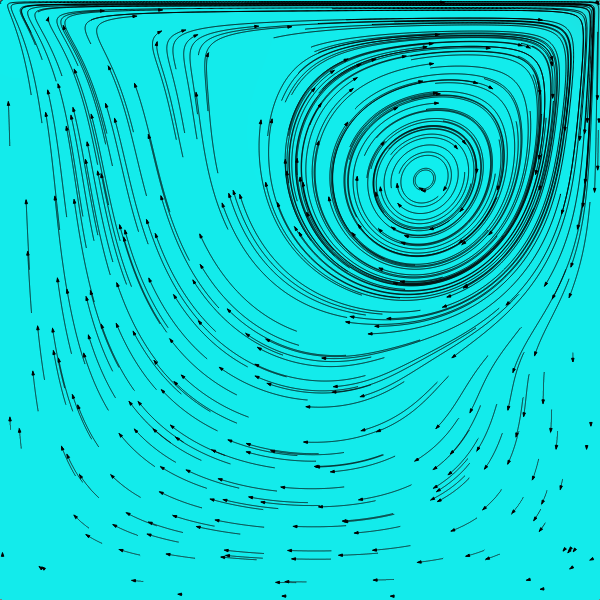
\includegraphics[scale = 0.28]{screenshots/re-1000-512-04758.png}
				\caption{$t=4.758$}
			\end{subfigure}
			\caption{simulierte Zeitevolution der Strömungslinien und des Druckfeldes für $Re=1000$ auf einem $512\times 512$-Gitter für verschiedene Zeitparameter $t$}
			\label{fig:time re 1000 1}
		\end{figure}

		\begin{figure}[!htb]
			\centering
			\begin{subfigure}[b]{.5\textwidth}
				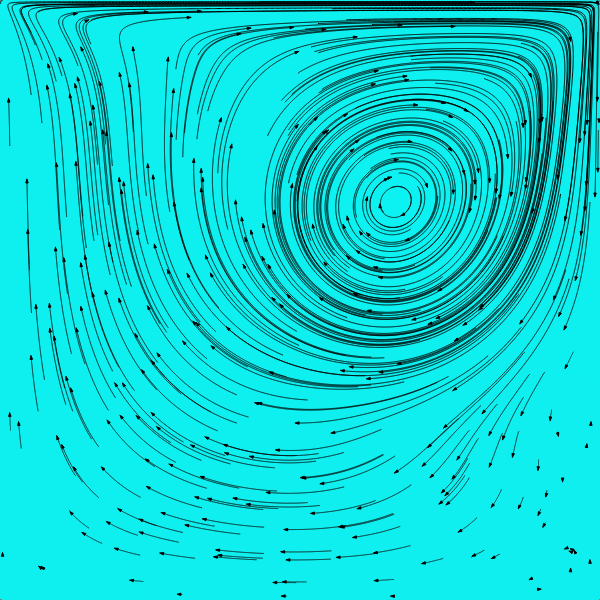
\includegraphics[scale = 0.28]{screenshots/re-1000-512-06482.png}
				\caption{$t=6.482$}
			\end{subfigure}%
			\begin{subfigure}[b]{.5\textwidth}
				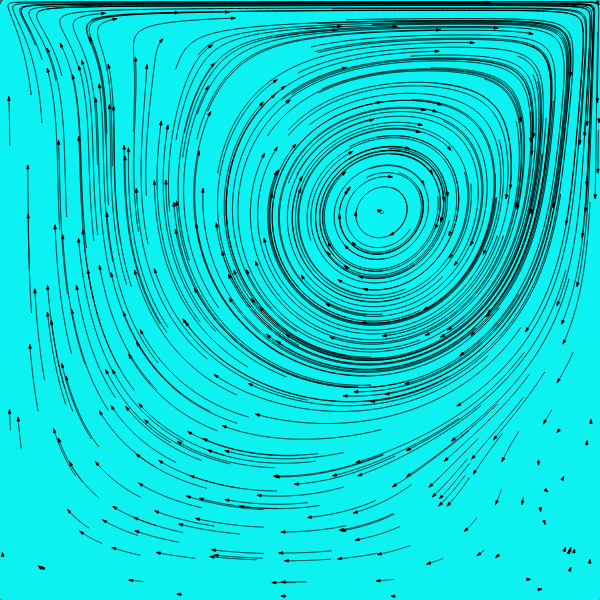
\includegraphics[scale = 0.28]{screenshots/re-1000-512-07612.png}
				\caption{$t=7.612$}
			\end{subfigure}

			\begin{subfigure}[b]{.5\textwidth}
				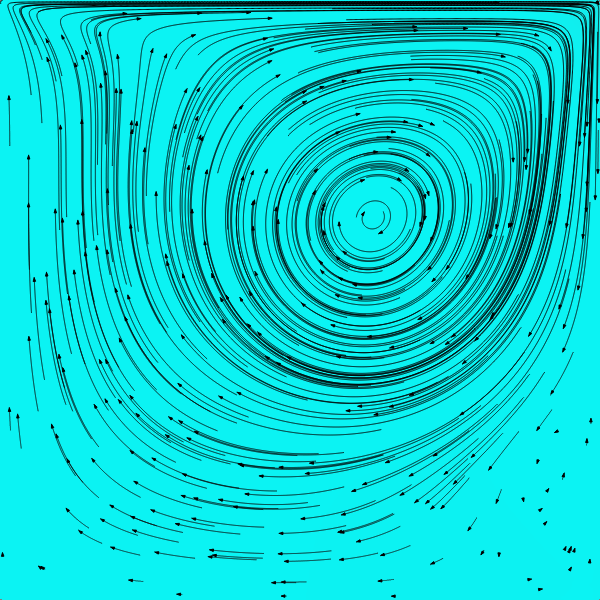
\includegraphics[scale = 0.28]{screenshots/re-1000-512-08419.png}
				\caption{$t=8.419$}
			\end{subfigure}%
			\begin{subfigure}[b]{.5\textwidth}
				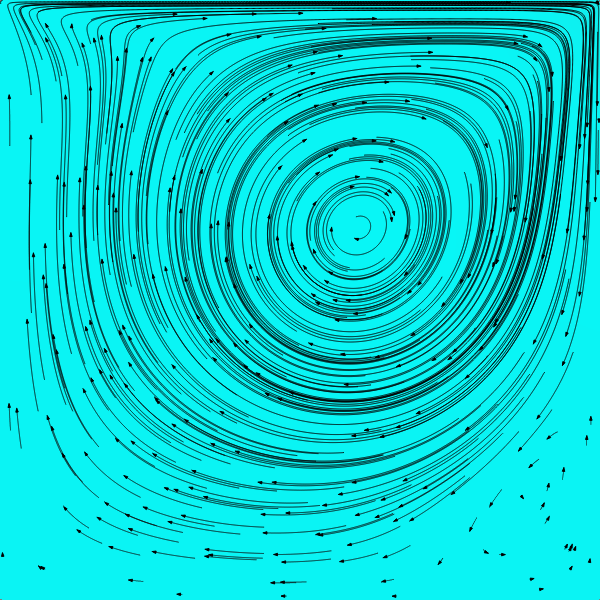
\includegraphics[scale = 0.28]{screenshots/re-1000-512-10164.png}
				\caption{$t=10.164$}
			\end{subfigure}

			\begin{subfigure}[b]{.5\textwidth}
				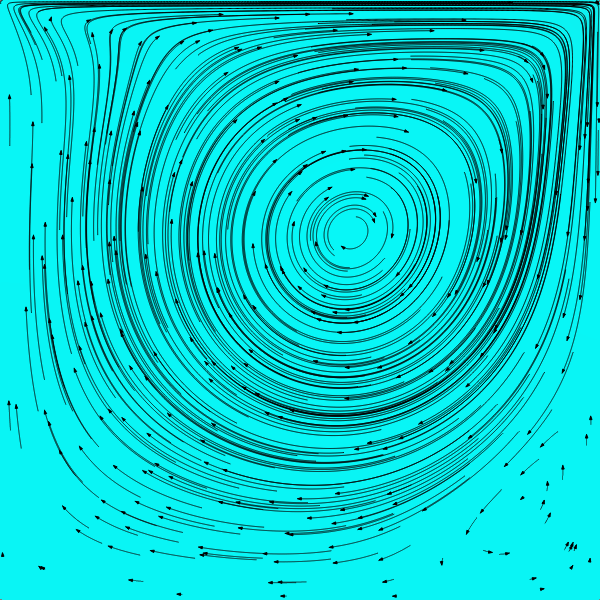
\includegraphics[scale = 0.28]{screenshots/re-1000-512-11408.png}
				\caption{$t=11.408$}
			\end{subfigure}%
			\begin{subfigure}[b]{.5\textwidth}
				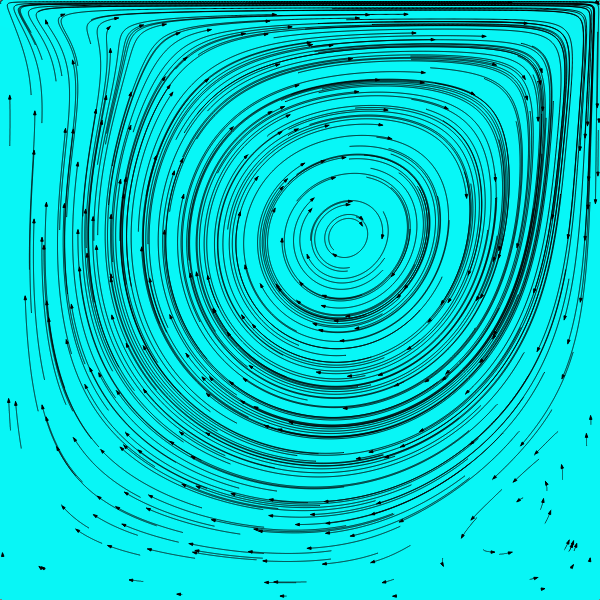
\includegraphics[scale = 0.28]{screenshots/re-1000-512-12475.png}
				\caption{$t=12.475$}
			\end{subfigure}
			\caption{simulierte Zeitevolution der Strömungslinien und des Druckfeldes für $Re=1000$ auf einem $512\times 512$-Gitter für verschiedene Zeitparameter $t$}
			\label{fig:time re 1000 2}
		\end{figure}

	% subsection einfluss_der_reynoldszahl (end)


	\subsection{Untersuchung von rechtwinkligen Geometrien} % (fold)
	\label{sub:untersuchung_von_rechtwinkligen_geometrien}
	
		Im Folgenden werden wieder nur stationäre Zustände des Strömungsfeldes betrachtet.
		Dabei sei wieder $Re=100$ und die Größe des Gitters $64\times 64$.

		Die Simulationen für rechteckige Boxgeometrien sind in den Abbildungen \ref{fig:box 1} und \ref{fig:box 2} zu sehen.
		Es wird deutlich, dass sich durch die Wahl von $a\geq b$ die Lösung qualitativ kaum von der ursprünglichen Lösung unterscheidet.
		Der entstehende Wirbel scheint einfach mit dem Parameter $a$ skaliert zu werden.
		Ein wesentlicher Unterschied besteht hier in der Deformation des Wirbels, welche aber eine logische Konsequenz aus der Änderung der Boxgeometrie ist.

		\begin{figure}[!hptb]
			\centering
			\begin{subfigure}[b]{.5\textwidth}
				\center
				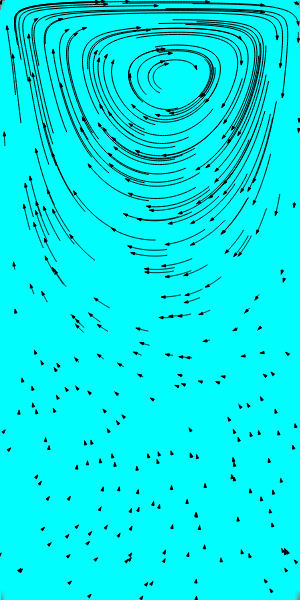
\includegraphics[scale = 0.30]{screenshots/box-05-10.png}
				\caption{$a=0.5, b=1.0$}
			\end{subfigure}%
			\begin{subfigure}[b]{.5\textwidth}
				\center
				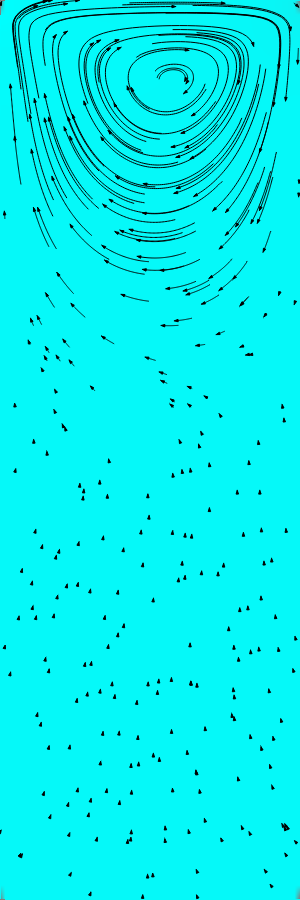
\includegraphics[scale = 0.30]{screenshots/box-05-15.png}
				\caption{$a=0.5, b=1.5$}
			\end{subfigure}
			\caption{Simulation des stationären Strömungsfeldes für verschiedene Boxgeometrien}
			\label{fig:box 1}
		\end{figure}

		Für den Fall $a<b$ ist aber nun in Abbildung \ref{fig:box 1} eine etwas andere Strömung zu sehen.
		Der gesamte Wirbel wird weder deformiert noch skaliert.
		Er behält in etwa seine Größe bei.

		\begin{figure}[!hptb]
			% \centering
			\begin{subfigure}[b]{.5\textwidth}
				\center
				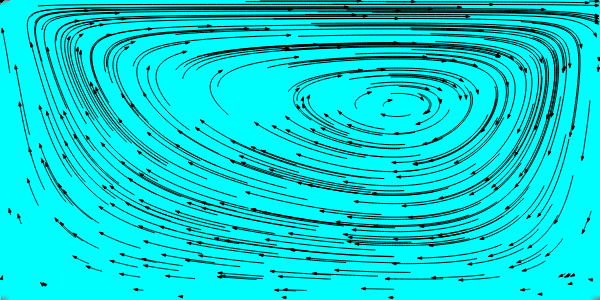
\includegraphics[scale = 0.32]{screenshots/box-10-05.png}
				\caption{$a=1.0, b=0.5$}
			\end{subfigure}

			\begin{subfigure}[b]{.5\textwidth}
				\center
				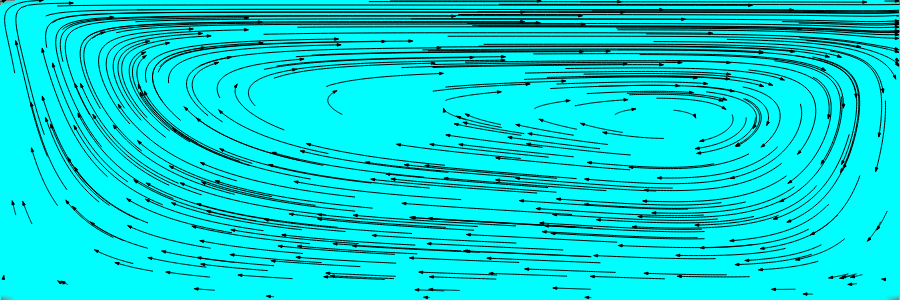
\includegraphics[scale = 0.32]{screenshots/box-15-05.png}
				\caption{$a=1.5, b=0.5$}
			\end{subfigure}
			\caption{Simulation des stationären Strömungsfeldes für verschiedene Boxgeometrien}
			\label{fig:box 2}
		\end{figure}

	% subsection untersuchung_von_rechtwinkligen_geometrien (end)


	\subsection{Periodische Anregung} % (fold)
	\label{sub:periodische_anregung}

		Für diesen Versuchsteil wurde für die Randgeschwindigkeit die folgende periodische Funktion verwendet.
		\[ \cos 3t \]
		Dabei beschreibt $t$ wieder den Zeitparameter der Simulation.
		Die Ergebnisse sind in den Abbildungen \ref{fig:periodic 1} und \ref{fig:periodic 2} zu sehen.
	
		\begin{figure}[!htb]
			\centering
			\begin{subfigure}[b]{.5\textwidth}
				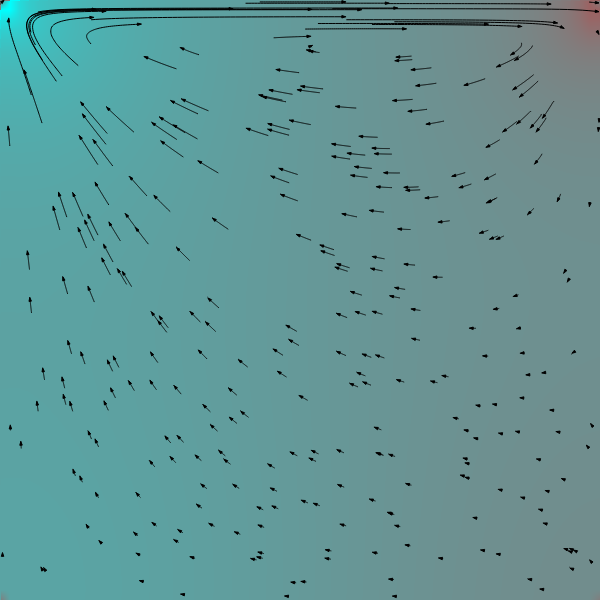
\includegraphics[scale = 0.28]{screenshots/periodic-00063.png}
				\caption{$t=0.063$}
			\end{subfigure}%
			\begin{subfigure}[b]{.5\textwidth}
				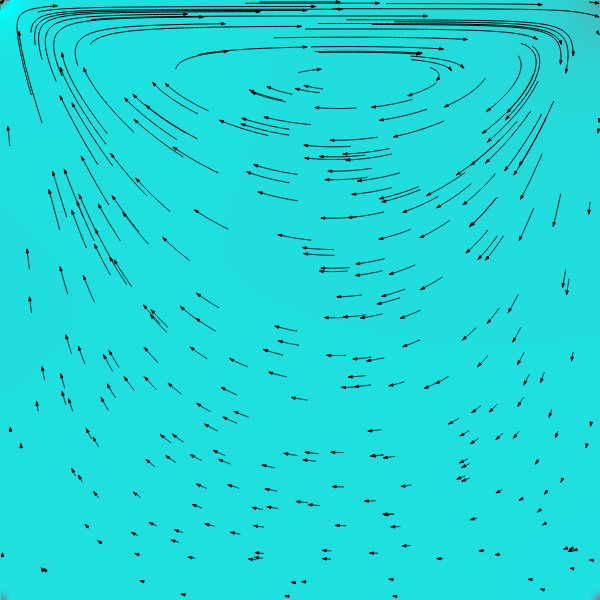
\includegraphics[scale = 0.28]{screenshots/periodic-00286.png}
				\caption{$t=0.286$}
			\end{subfigure}

			\begin{subfigure}[b]{.5\textwidth}
				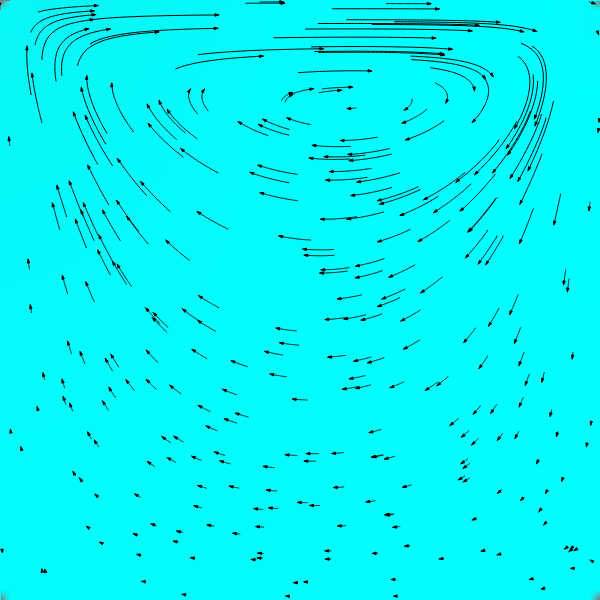
\includegraphics[scale = 0.28]{screenshots/periodic-00507.png}
				\caption{$t=0.507$}
			\end{subfigure}%
			\begin{subfigure}[b]{.5\textwidth}
				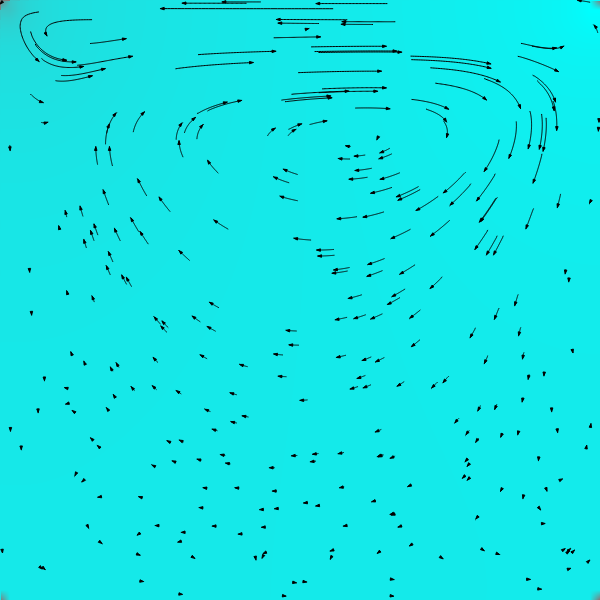
\includegraphics[scale = 0.28]{screenshots/periodic-00702.png}
				\caption{$t=0.702$}
			\end{subfigure}

			\begin{subfigure}[b]{.5\textwidth}
				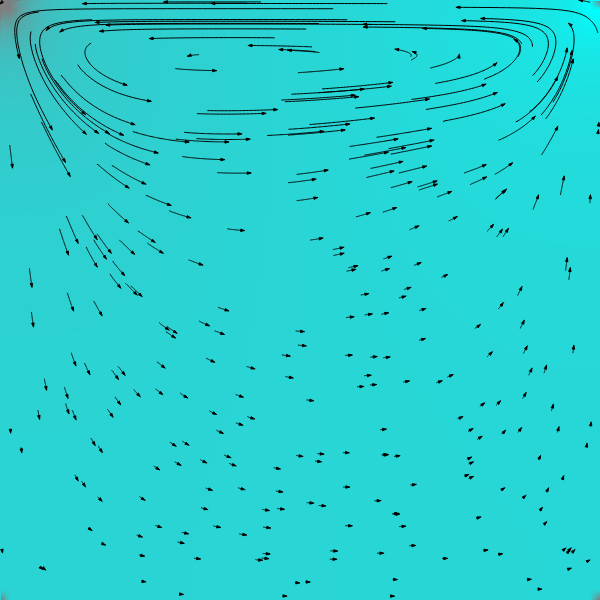
\includegraphics[scale = 0.28]{screenshots/periodic-00944.png}
				\caption{$t=0.944$}
			\end{subfigure}%
			\begin{subfigure}[b]{.5\textwidth}
				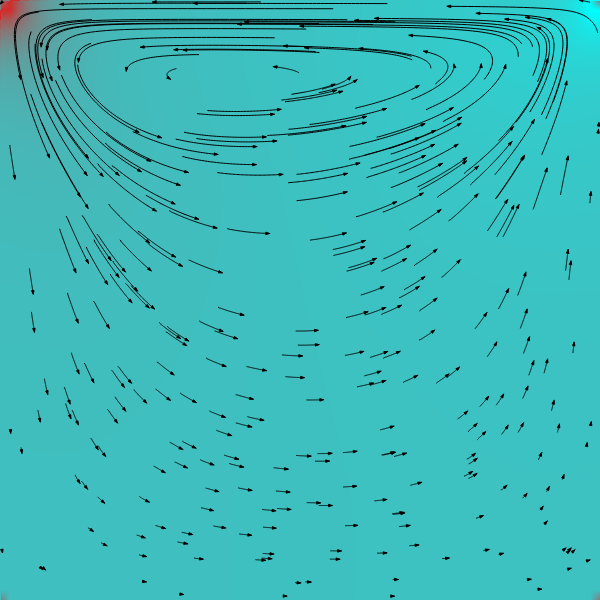
\includegraphics[scale = 0.28]{screenshots/periodic-01162.png}
				\caption{$t=1.162$}
			\end{subfigure}
			\caption{simulierte Zeitevolution Strömungslinien und des Druckfeldes, welche periodisch angeregt werden, für verschiedene Zeitparameter $t$}
			\label{fig:periodic 1}
		\end{figure}

		\begin{figure}[!htb]
			\centering
			\begin{subfigure}[b]{.5\textwidth}
				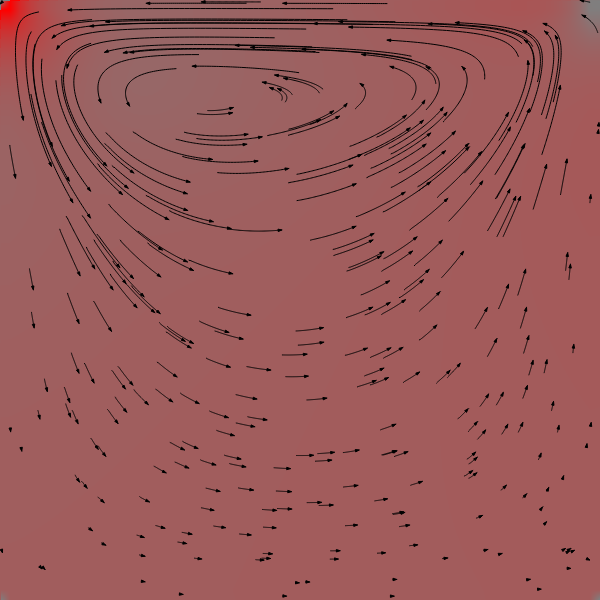
\includegraphics[scale = 0.28]{screenshots/periodic-01442.png}
				\caption{$t=1.442$}
			\end{subfigure}%
			\begin{subfigure}[b]{.5\textwidth}
				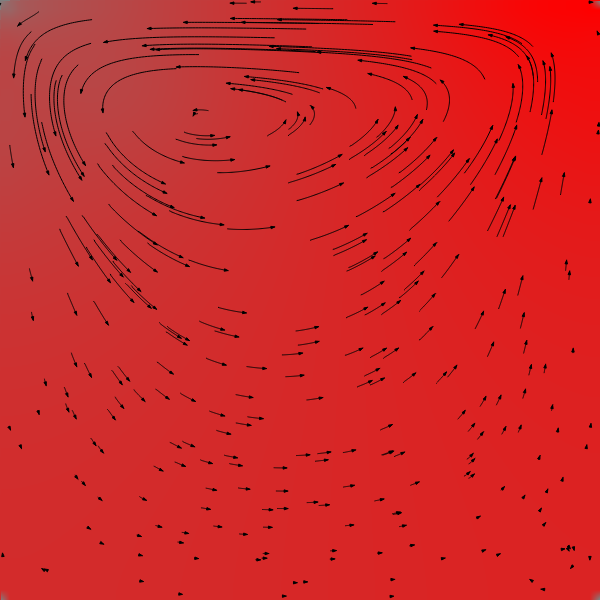
\includegraphics[scale = 0.28]{screenshots/periodic-01606.png}
				\caption{$t=1.606$}
			\end{subfigure}

			\begin{subfigure}[b]{.5\textwidth}
				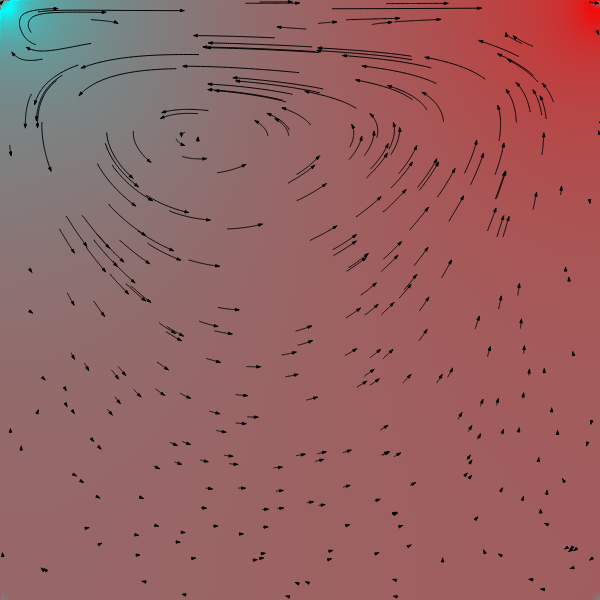
\includegraphics[scale = 0.28]{screenshots/periodic-01735.png}
				\caption{$t=1.735$}
			\end{subfigure}%
			\begin{subfigure}[b]{.5\textwidth}
				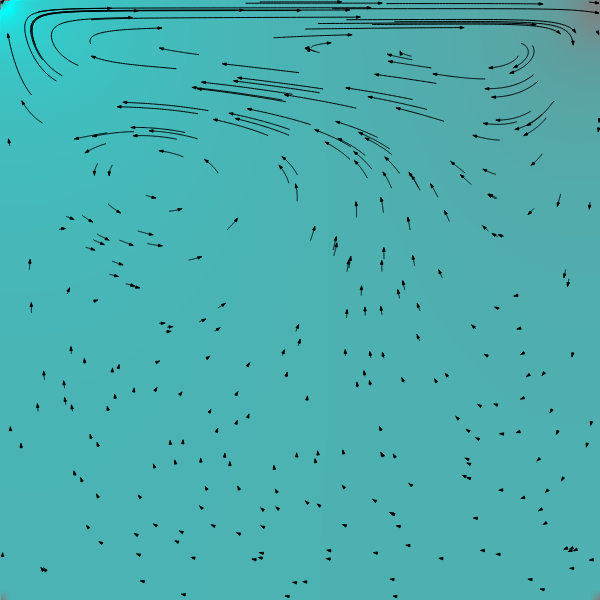
\includegraphics[scale = 0.28]{screenshots/periodic-01921.png}
				\caption{$t=1.921$}
			\end{subfigure}

			\begin{subfigure}[b]{.5\textwidth}
				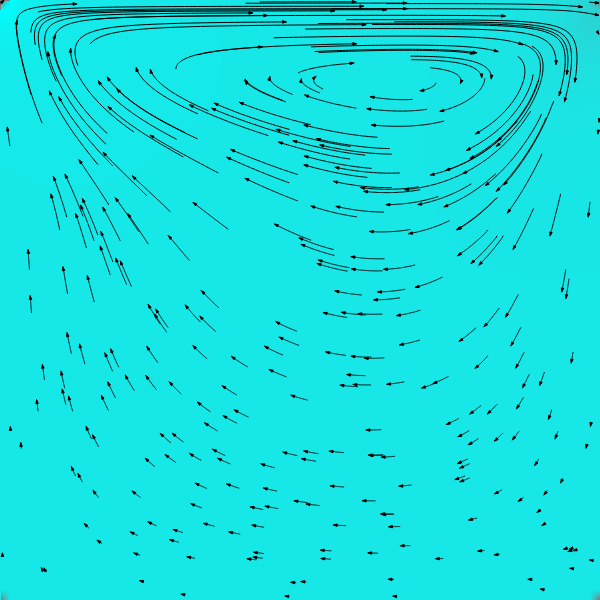
\includegraphics[scale = 0.28]{screenshots/periodic-02299.png}
				\caption{$t=2.299$}
			\end{subfigure}%
			\begin{subfigure}[b]{.5\textwidth}
				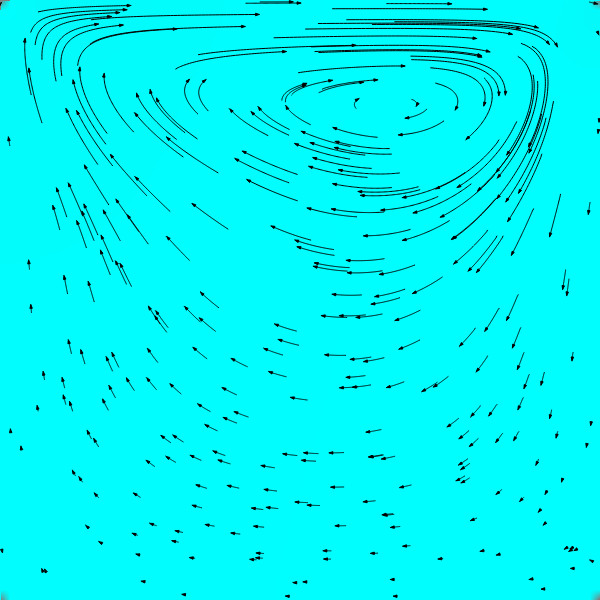
\includegraphics[scale = 0.28]{screenshots/periodic-02573.png}
				\caption{$t=2.573$}
			\end{subfigure}
			\caption{simulierte Zeitevolution Strömungslinien und des Druckfeldes, welche periodisch angeregt werden, für verschiedene Zeitparameter $t$}
			\label{fig:periodic 2}
		\end{figure}

		Wie zu erwarten war wechseln die Drehrichtungen des Wirbels, je nachdem in welche Richtung die Randgeschwindigkeit zeigt.
		Es ist wichtig zu bemerken, dass beim Wechsel der Geschwindigkeitsrichtung ein enormer Druckanstieg zu beobachten ist.

	% subsection periodische_anregung (end)

% section simulation_und_ergebnisse (end)